\newcommand{\gatedistancein}{3pt}
\newcommand{\gatedistanceinand}{2pt}
\tikzset{
%AUTOMATA & PETRI NET STUFF
every state/.style={minimum size=7pt,inner sep=1pt, initial text={}},
every place/.style={minimum size=7pt,inner sep=1.2pt},
every token/.style={minimum size=2pt,inner sep=1.2pt},
every transition/.style={minimum size=9pt,inner sep=1.8pt},
%GLOBAL GRAPH STUFF
source/.style={draw,circle,fill=white,
  minimum size=4mm,
  inner sep=0pt},
sink/.style={draw,circle,double,fill=white,
  minimum size=3mm,
  inner sep=0pt},
%AND GATE
agate/.style={draw,rectangle,
  minimum size=3mm,
  inner sep=0pt,
  fill=white,
  postaction={path picture={% 
    \draw[black]
      ([yshift=\gatedistanceinand]path picture bounding box.south) --
      ([yshift=-\gatedistanceinand]path picture bounding box.north) ;}}},
%
%ACTION
block/.style = {rectangle, draw=gray, align=center, fill=white, rounded corners=0.1cm,
  minimum size=5mm, inner sep=2pt},
prenode/.style = {minimum size=9pt,inner sep=2pt, font=\Large},
% 
% ORGATE
ogate/.style = {
  diamond, draw, fill=white,
  minimum size=4mm,
  inner sep=0pt,
  postaction={path picture={% 
      \draw[black]
      ([yshift=\gatedistancein]path picture bounding box.south) -- ([yshift=-\gatedistancein]path picture bounding box.north)
      ([xshift=-\gatedistancein]path picture bounding box.east) -- ([xshift=\gatedistancein]path picture bounding box.west)
      ;}}},
% 
% ogate or agate
anygate/.style = {circle, draw, fill=white,
  minimum size=4mm,
    inner sep=0pt,
    postaction={path picture={% 
    \draw[black]
    ([xshift=-\gatedistancein,yshift=\gatedistancein]path picture bounding box.south east) --
    ([xshift=\gatedistancein,yshift=-\gatedistancein]path picture bounding box.north west)
    ([xshift=-\gatedistancein,yshift=-\gatedistancein]path picture bounding box.north east) --
    ([xshift=\gatedistancein,yshift=\gatedistancein]path picture bounding box.south west)
    ;}}},
%
% DOTS
elli/.style = {draw,densely dotted,-},
% 
% LINES
line/.style = {draw,->, rounded corners=0.07cm,>=latex},
nline/.style = {draw,semithick, ->},
pline/.style = {draw,->,>=latex},
node distance=1cm and 0.7cm,
baseline=(current  bounding  box.center),
mycfsm/.style={
  font=\footnotesize,
  initial where=above,
  ->,>=stealth,auto, node distance=1cm and 1cm,
  scale=1, every node/.style={transform shape},
  baseline=(current  bounding  box.center)
},
mypetri/.style={
  font=\footnotesize,
  baseline=(current  bounding  box.center)
},
silentrans/.style = {rectangle, draw=black, align=center, fill=black,
  minimum height=1pt,
  minimum width=15pt,
  inner sep=1.5pt
},
smallthings/.style={
  ->,>=stealth',shorten >=1pt,auto,node distance=2cm,
  semithick,
  scale=0.6, every node/.style={transform shape}
},
smallglobal/.style={
  node distance=1cm and 0.8cm, semithick, scale=0.8, every node/.style={transform shape}
},
smallmacro/.style={
  node distance=1cm and 0.8cm, semithick, scale=0.5, every node/.style={transform shape}
},
icts/.style={
  >=latex',line join=bevel,scale=0.5, every node/.style={transform shape},font=\Large
},
smallmacro/.style={
  node distance=1cm and 0.8cm, semithick, scale=0.5, every node/.style={transform shape}
},
process/.style={rectangle, draw, fill=white, drop shadow,
  text centered, minimum height=5em
},
bigar/.style={
  draw,very thick, ->
},
bignoar/.style={
  draw,very thick, ->
},
vecArrow/.style = {thick, decoration={markings,mark=at position
    1 with {\arrow[semithick]{open triangle 60}}},
  double distance=1.4pt, shorten >= 5.5pt,
  preaction = {decorate},
  postaction = {draw,line width=1.4pt, white,shorten >= 4.5pt}
},
local/.style={rectangle, draw, fill=white, drop shadow,
  text centered, rounded corners, minimum height=5em
},
choreo/.style={rectangle, draw, fill=white, drop shadow,
  text centered, rounded corners, minimum height=5em
},
to*/.style={
  shorten >=.25em,#1-to,
  to path={-- node[inner sep=0pt,at end,sloped] {${}^*$} (\tikztotarget) \tikztonodes}
},
to*/.default=
}


%%%%%%%%%%%%%%%%%%%%%%%%%%%%%%%%%%%%%%%%%%%%%%%%%%%%%%%%%%%%%%%%%%%%%%%%%%%%%%%%%%%%%%%%%%%%%%%%%%
% CONCUR 12
%%%%%%%%%%%%%%%%%%%%%%%%%%%%%%%%%%%%%%%%%%%%%%%%%%%%%%%%%%%%%%%%%%%%%%%%%%%%%%%%%%%%%%%%%%%%%%%%%%

\newcommand{\singleN}[1]{#1}

\newcommand{\onekid}[1]
{
  \begin{tikzpicture}
    \node (top) {\ensuremath{\nodeTN}};
    \node [below of=top] (kid) {\ensuremath{#1}};
    \draw[line] (top) -- (kid);
  \end{tikzpicture}
}


\newcommand{\onekidR}[2]
{
 \begin{tikzpicture}
    \node (top) {\ensuremath{#1}};
    \node [below of=top] (kid) {\ensuremath{#2}};
    \draw[line] (top) -- (kid);
  \end{tikzpicture}
}


\newcommand{\twokids}[2]
{
  \begin{tikzpicture}[node distance=1.2cm and 1.2cm]
    \node (top) {\ensuremath{\nodeTN}};
    \node [below left of=top] (kid1) {\ensuremath{#1}};
    \node [below right of=top] (kid2) {\ensuremath{#2}};
    %
    \draw[line] (top) -- (kid1);
    \draw[line] (top) -- (kid2);
  \end{tikzpicture}
}
  
\newcommand{\twokidsR}[3]
{
  \begin{tikzpicture}[node distance=1.2cm and 1.2cm]
    \node (top) {\ensuremath{#1}};
    \node [below left of=top] (kid1) {\ensuremath{#2}};
    \node [below right of=top] (kid2) {\ensuremath{#3}};
    %
    \draw[line] (top) -- (kid1);
    \draw[line] (top) -- (kid2);
  \end{tikzpicture}
}

%%%%%%%%%%%%%%%%%%%%%%%%%%%%%%%%%%%%%%%%%%%%%%%%%%%%%%%%%%%%%%%%%%%%%%%%%%%%%%%%%%%%%%%%%%%%%%%%%%
% CFSMs
%%%%%%%%%%%%%%%%%%%%%%%%%%%%%%%%%%%%%%%%%%%%%%%%%%%%%%%%%%%%%%%%%%%%%%%%%%%%%%%%%%%%%%%%%%%%%%%%%%

\newcommand{\oneNode}[1]{
  \begin{tikzpicture}
    \node [block] (in) {$#1$};
  \end{tikzpicture}
}


%% IN TEXT%%%%%%%%%%%%%%%%%%%%%%%%%%%%%%%%%%
% \newcommand{\pargate}{\andgateG \,}
% \newcommand{\chgate}{\orgateG \,}
% \newcommand{\source}{\sourceG \,}
% \newcommand{\sink}{\sinkG \,}

\newcommand{\sourceG}{
  
\begin{tikzpicture}[smallglobal,baseline=-.5ex, scale=0.6, every node/.style={transform shape}]
  \node [source] (src) {};
\end{tikzpicture}
}

\newcommand{\sinkG}{
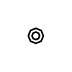
\begin{tikzpicture}[smallglobal,baseline=-.5ex, scale=0.6, every node/.style={transform shape}]
  \node [sink] (src) {};
\end{tikzpicture}
}

\newcommand{\orgateG}{
\begin{tikzpicture}[smallglobal,baseline=-.5ex, scale=0.75, every node/.style={transform shape}]
  \node [ogate] (o) {};
\end{tikzpicture}
}

\newcommand{\andgateG}{
\begin{tikzpicture}[smallglobal,baseline=-.5ex, scale=0.75, every node/.style={transform shape}]
  \node [agate] (o) {};
\end{tikzpicture}
}

\newcommand{\anygateG}{

\begin{tikzpicture}[smallglobal,baseline=-.5ex, scale=0.75, every node/.style={transform shape}]
  \node [anygate] (o) {};
\end{tikzpicture}
}

%%%%%%%%%%%%%%%%%%%%%%%%%%%%%%%%%%%%%%%%%%%%%
\newcommand{\TITOdistv}{0.4cm}
\newcommand{\TITOdisth}{0.25cm}
\newcommand{\TITOscale}{0.8}

\newcommand{\TOend}[1]{
  \begin{tikzpicture}[node distance=\TITOdistv and \TITOdisth, scale=\TITOscale, every node/.style={transform shape}]
    \node  (ti) at (0,0) {$#1$};
    \node [sink, right=of ti,scale=0.8,xshift=2pt] (lab) {};
    % 
    \path [line] (ti) -- (lab);
  \end{tikzpicture}
}

\newcommand{\TIstart}[1]{
  \begin{tikzpicture}[node distance=\TITOdistv and \TITOdisth, scale=\TITOscale, every node/.style={transform shape}]
    \node [source,scale=0.8] (ti) at (0,0) {};
    \node [right=of ti,xshift=2pt] (lab) {$#1$};
    % 
    \path [line] (ti) -- (lab);
  \end{tikzpicture}
}

\newcommand{\TOTIsequence}[2]{
  \begin{tikzpicture}[node distance=\TITOdistv and \TITOdisth, scale=\TITOscale, every node/.style={transform shape}]
    \node  (ti) at (0,0) {$#1$};
    \node [right=of ti] (lab) {$#2$};
    % 
    \path [line] (ti) -- (lab);
  \end{tikzpicture}
}


\newcommand{\TIfigure}[5]{
  \begin{tikzpicture}[node distance=\TITOdistv and \TITOdisth, scale=\TITOscale, every node/.style={transform shape}]
    \node (lab) at (0,0) {$#1$};
    \node [#5, left=of lab,scale=0.8] (gate) {};
    % 
    \node [left=of gate] (ei) {$#3$};
    \node [above=of gate] (e1)  at (gate -| ei) {$#2$};
    \node [below=of gate] (ek) at (gate -| ei) {$#4$};
    % 
    \path [line] (gate) -- (lab);
    \path [line] (e1) -| (gate);
    \path [line] (ek) -| (gate);
    \path [line] (ei) -- (gate);
    \path [elli] (e1) -- (ei);
    \path [elli] (ei) -- (ek);
  \end{tikzpicture}
}



\newcommand{\TOfigure}[5]{
  \begin{tikzpicture}[node distance=\TITOdistv and \TITOdisth, scale=\TITOscale, every node/.style={transform shape}]
    \node (lab) at (0,0) {$#1$};
    \node [#5, right=of lab,scale=0.8] (gate) {};
    % 
    \node [right=of gate] (ei) {$#3$};
    \node [above=of gate] (e1)  at (gate -| ei) {$#2$};
    \node [below=of gate] (ek) at (gate -| ei) {$#4$};
    %
    \path [line] (lab) -- (gate);
    \path [line] (gate) |- (e1);
    \path [line] (gate) |- (ek);
    \path [line] (gate) -- (ei);
    \path [elli] (e1) -- (ei);
    \path [elli] (ei) -- (ek);
  \end{tikzpicture}
}

\newcommand{\threeout}[6][1]{
  \begin{tikzpicture}
    \node [block] (e1)  at (0,0)    {$#4$};
    \node [block] (ei)  at (0,-.5)  {$#5$};
    \node [block] (en)  at (0,-1)   {$#6$};
    \node [#2] (gtop)   at (-1,-.5) {};
    \node [block] (inp) at (-4*#1,-.5) {$#3$};
    % 
    \path [line] (inp) -- (gtop);
    \path [line] (gtop) -- (ei);
    \path [line] (gtop) |- (e1);
    \path [line] (gtop) |- (en);
    \path [elli] (e1) -- (ei);
    \path [elli] (ei) -- (en);
  \end{tikzpicture}
}


\newcommand{\oneout}[3][1]
{
  \begin{tikzpicture}[node distance=#1cm and #1cm]
    \node [block] (inp) {$#2$};
    \node [block, right=0.3cm and 0.3cm of inp] (e) {$#3$};
      
    \path [line] (inp) -- (e);
  \end{tikzpicture}
}

\newcommand{\onein}[3][1]{\oneout[#1]{#2}{#3}}







\newcommand{\threein}[6][1]{
  \begin{tikzpicture}
    \node [block] at (0,0)  (e1) {$#3$};
    \node [block] at (0,-.5) (ei) {$#4$};
    \node [block] at (0,-1)  (en) {$#5$};
    \node [#2]    at (1.7*#1,-.5) (gtop) {};
    \node [block] at (3*#1,-.5) (outp) {$#6$};
    % 
    \path [line] (gtop) -- (outp);
    \path [line] (ei) -- (gtop);
    \path [line] (e1) -| (gtop);
    \path [line] (en) -| (gtop);
    \path [elli] (e1) -- (ei);
    \path [elli] (ei) -- (en);
  \end{tikzpicture}
}


\newcommand{\threeinL}[6][1]{
  \begin{tikzpicture}
    \node [block] at (0,0)  (e1) {$#3$};
    \node [block] at (0,-.5) (ei) {$#4$};
    \node [block] at (0,-1)  (en) {$#5$};
    \node [#2]    at (1.7,-.5) (gtop) {};
    \node [block] at (3*#1,-.5) (outp) {$#6$};
    % 
    \path [line] (gtop) -- (outp);
    \path [line] (ei) -- (gtop);
    \path [line] (e1) -| (gtop);
    \path [line] (en) -| (gtop);
    \path [elli] (e1) -- (ei);
    \path [elli] (ei) -- (en);
  \end{tikzpicture}
}


\newcommand{\convexpath}[2]{
  [   
  create hullnodes/.code={
    \global\edef\namelist{#1}
    \foreach [count=\counter] \nodename in \namelist {
      \global\edef\numberofnodes{\counter}
      \node at (\nodename) [draw=none,name=hullnode\counter] {};
    }
    \node at (hullnode\numberofnodes) [name=hullnode0,draw=none] {};
    \pgfmathtruncatemacro\lastnumber{\numberofnodes+1}
    \node at (hullnode1) [name=hullnode\lastnumber,draw=none] {};
  },
  create hullnodes
  ]
  ($(hullnode1)!#2!-90:(hullnode0)$)
  \foreach [
  evaluate=\currentnode as \previousnode using \currentnode-1,
  evaluate=\currentnode as \nextnode using \currentnode+1
  ] \currentnode in {1,...,\numberofnodes} {
    -- ($(hullnode\currentnode)!#2!-90:(hullnode\previousnode)$)
    let \p1 = ($(hullnode\currentnode)!#2!-90:(hullnode\previousnode) - (hullnode\currentnode)$),
    \n1 = {atan2(\x1,\y1)},
    \p2 = ($(hullnode\currentnode)!#2!90:(hullnode\nextnode) - (hullnode\currentnode)$),
    \n2 = {atan2(\x2,\y2)},
    \n{delta} = {-Mod(\n1-\n2,360)}
    in 
    {arc [start angle=\n1, delta angle=\n{delta}, radius=#2]}
  }
  -- cycle
}

%%% Local Variables: 
%%% mode: latex
%%% TeX-master: "main"
%%% End: